% ---------------------------------------------------------------------
% LaTeX template for abstract submission to EUROMECH Colloquium #609
%
% 7-aug-2019 m. uhlmann
% ---------------------------------------------------------------------
\documentclass[a4paper,11pt]{article}

%\usepackage[latin1]{inputenc}
%\usepackage[T1]{fontenc}
\usepackage[utf8]{inputenc}
\usepackage{subcaption}
\usepackage[paper=a4paper,left=28mm,right=28mm,top=25mm,bottom=30mm]{geometry}
\usepackage[pdftex,colorlinks=true,linkcolor=blue,citecolor=blue,urlcolor=blue]{hyperref}
\usepackage{graphicx}
\usepackage{epstopdf}
\usepackage[sort&compress,round]{natbib}
\usepackage{doi}
\usepackage{tikz}
 \usetikzlibrary{fit,arrows.meta,shapes.arrows}
\usepackage{fancyhdr}
\pagestyle{fancy}
\setlength{\headheight}{30pt}
\fancyhfoffset{32pt}
\lhead{}
\chead{%\bf
  \sffamily
  \parbox[t]{.96\linewidth}{
  \small
    ~ EUROMECH Colloquium 654 
    ``Bio-Inspired Fluid-Structure Interaction'' ~~~~~~~~~~~~
    9-11 July 2025, Vienna, Austria
  }
}
\rhead{}

\begin{document}

\vspace{-1.0cm}

\epstopdfsetup{suffix=}
%----------------------------------------------------------------------
\title{Flexible foil dynamics under shear flow: stabilization through spanwise modulation.}

\author{Nicolás Silin $^1$\and  Pablo Cobelli$^2$ \and Juan D'Adamo$^{3}$\\
  $^1$ Instituto Balseiro, CNEA, CONICET,  8400 Bariloche, Argentina. \\
  $^2$ Universidad de Buenos Aires, Facultad de Ciencias Exactas y Naturales,\\  IFIBA, CONICET,   Buenos Aires,  Argentina.\\
  $^3$ Universidad de Buenos Aires, Facultad de Ingenier\'ia, \\LFD, CONICET,Buenos Aires, Argentina.
}
\date{}
\maketitle
We study the interaction between shear flows and the mechanics of an elastic flexible foil. We employ a paper sheet, uniform in the spanwise direction,  subjected to a flow from a wind tunnel.

First, we characterize the coupled dynamics of elasticity and shear instabilities, investigating the relationship between the foil's deformations, vibrations, and flow properties associated with Kelvin-Helmholtz instabilities.

Second, we explore 3D modulation by introducing spanwise geometric modifications (cuts) in the foil. These alterations strongly interact with the flow,  stabilizing the fluid-structure dynamics. To achieve these objectives, we employ   fast-camera imaging combined with an optical profilometric technique [Cobelli:2009p63] to analyze the elastic deformations.




	
	

\begin{figure}
	
\begin{subfigure}[b]{.5\textwidth}
\input{modo_elastico.tikz}
\subcaption{Dshape with flexible foils in the wind tunnel. }	
\end{subfigure}	
\begin{subfigure}[b]{.5\textwidth}
	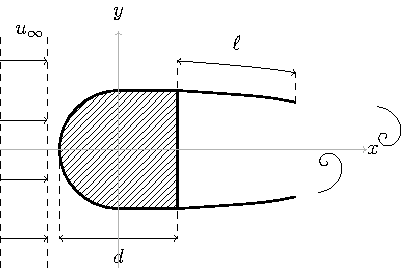
\includegraphics[width=\textwidth]{./setup_scheme}
	\subcaption{Scheme of the flow and solid configuration. }
\end{subfigure}
\label{fig}
\vspace{-0.5cm}
\caption{}\label{fig_setup}
\end{figure}

% -----------------------------------------------------------------------
\bibliography{/home/juan/Documents/bibtex/citas.bib}
\bibliographystyle{plainnat}
\setlength{\bibsep}{.5ex}
%
% There are two ways to produce a list of references. 
%
% A) include a bibtex file:
%
% \bibliography{/home/uhlmann/TEX/bib/books.bib}
%
% B) insert the bibliography items directly:
%
 
%----------------------------------------------------------------------
\end{document}
% ---------------------------------------------------------------------